\section{Generalized Linear Models} 

  Remember the linear model looked like this, where we use the conventional $\beta$ notation to represent parameters. 
  \begin{equation}
    Y = X^T \beta + \epsilon, \;\; \epsilon \sim N(0, \sigma^2 I)
  \end{equation}
  which implies that $Y \mid X \sim N(X^T \beta, \sigma^2 I)$. Basically, given $x$, I assume some distribution of $Y$, and the value of $x$ will help me guess what the mean of this distribution is. Note that we in here assume that only the mean depends on $X$. I could potentially have something crazy, like 
  \[Y \mid X \sim N(X^T \beta, (X^T \gamma) (X X^T + I))\]
  where the covariance will depend on $X$, too, but in this case we only assume that that mean is dependent on $X$. 
  \[Y \mid X \sim N(\mu(X), \sigma^2 I)\]
  where in the linear model, $\mu(X) = X^T \beta$. So, there are three assumptions we are making here: 
  \begin{enumerate}
    \item $Y \mid X$ is Gaussian. 
    \item $X$ only affects the mean of $Y \mid X$, written $\mathbb{E}[Y \mid X] = \mu(X)$. 
    \item $X$ affects the mean in a linear way, such that $\mu(X) = X^T \beta$. 
  \end{enumerate}
  So the two things we are trying to relax are: 
  \begin{enumerate}
    \item \textbf{Random Component}: the response variable $Y \mid X$ is continuous and normally distributed with mean $\mu = \mu(X) = \mathbb{E}[Y \mid X]$. 
    \item \textbf{Link}: I have a link that explains the relationship between the $X$ and the $\mu$, and this relationship is $\mu(X) = X^T \beta$. 
  \end{enumerate}
  So when talking about GLMs, we are not changing the fact that we have a linear function $X \mapsto X^T \beta$. However, we are going to assume that $Y \mid X$ now comes from a broader \textbf{family of exponential distributions}. Second, we are going to assume that there exists some \textbf{link function} $g$
  \[g(\mu(X)) = X^T \beta\]
  Admittedly, this is not the most intuitive way to think about it, since we would like to have $\mu(X) = f(X^T \beta)$, but here we just decide to call $f = g^{-1}$. Therefore, if I want to give you a GLM, I just need to give you two things: the conditional distribution $Y \mid X$, which can be any distribution in the exponential family, and the link function $g$. 

  We really only need this link function due to compatibility reasons. Say that $Y \mid X \sim \mathrm{Bern}(p)$. Then, $\mu(X) = \mathbb{E}[Y \mid X]$ always lives in $[0, 1]$, but $X^T \beta$ always lives in $\mathbb{R}$. We want our model to be realistic, and we can clearly see the problem shown in Figure \ref{fig:Bernoulli_GLM}. 

  \begin{figure}[H]
    \centering
    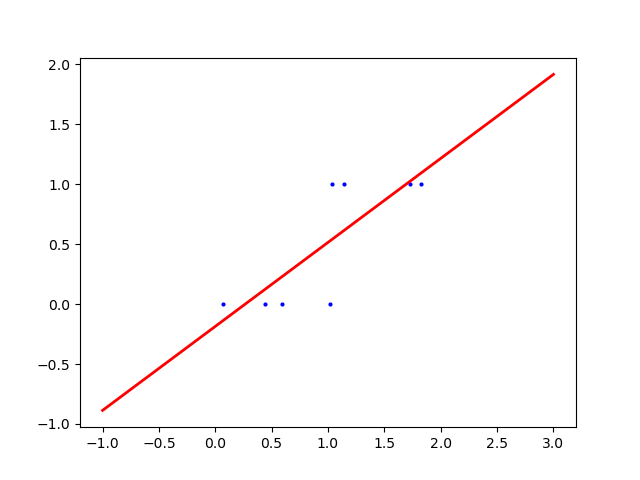
\includegraphics[scale=0.5]{img/GLM_bernoulli.png}
    \caption{Fitting a linear model for Bernoulli random variables will predict a mean that is outside of $[0, 1]$ when getting new datapoints. }
    \label{fig:Bernoulli_GLM}
  \end{figure}

  If $Y \mid X$ is some exponential distribution, then its support is always positive and so $\mu(X) > 0$. But if we stick to the old form of $\mu(X) = X^T \beta$, then $\mathrm{Im}(\mu) = \mathbb{R}$, which is not realistic when we predict negative values. Let's take a couple examples: 

  \begin{example}[Disease Epidemic]
    In the early stages of a disease epidemic, the rate at which new cases occur can often increase exponentially through time. Clearly, $\mu(X) = \mathbb{E}[Y \mid X]$ should be positive and we should have some sort of exponential trend. Hence, if $\mu(x)$ is the expected number of cases on data $x$, a model of the form 
    \begin{equation}
      \mu(x) = \gamma \exp (\delta x)
    \end{equation}
    seems appropriate, where $\gamma$ and $\delta$ are simply scaling factors. Clearly, $\mu(X)$ is not of the form $f(X^T \beta)$. So what I do is to transform $\mu$ in such a way that I can get something that is linear. 
    \begin{equation}
      \log(\mu(X)) = \log(\gamma) + \delta X
    \end{equation}
    which is now linear in $X$, of form $\beta_0 + \beta_1 X$. This will have some effects, but this is what needs to be done to have a genearlized linear model. Note that what I did to $\mu$ was take the log of it, and so the link function is $g = \log$, called the \textbf{log-link}. Now that we have chosen the $g$, we still need to choose what the conditional distribution $Y \mid X$ would be. This is determined by speaking with industry professionals, experience, and convenience. In this case, $Y$ is a count, and since this must be a discrete distribution. Since it is not bounded above, we think Poisson. 
  \end{example}

  \begin{example}[Prey Capture Rate]
    The rate of capture of preys, $Y$, by a hunting animal, tends to increase with increasing density of prey $X$, but eventually level off when the predator is catching as much as it can cope with. We want to find a perhaps concave function that levels off, and suitable model might be 
    \begin{equation}
      \mu(X) = \frac{\alpha X}{h + X}
    \end{equation}
    where $\alpha$ represents the maximum capture rate, and $h$ represents the prey density at which the capture rate is half the maximum rate. Again, we must find some transformation $g$ that turns this into a linear function of $X$, and what we can do it use the \textbf{reciprocal-link}. 
    \begin{equation}
      \frac{1}{\mu(X)} = \frac{h + X}{\alpha X} = \frac{h}{\alpha} \frac{1}{X} + \frac{1}{\alpha}
    \end{equation}
    The standard deviation of capture rate might be approximately proportional to the mean rate, suggesting the use of a Gamma distribution for the response. 
  \end{example}

  \begin{example}[Kyphosis Data]
    The Kyphosis data consist of measurements on $81$ children following corrective spinal surgery. The binary response variable, Kyphosis, indicates the presence or absence of a postoperative deforming. The three covariates are: age of the child in months, number of the vertebrae involved in the operation, and the start of the range of the vertebrae involved. The response variable is binary so there is no choice: $Y \mid X$ is Bernoulli with expected value $\mu(X) \in (0, 1)$. We cannot write $\mu(X) = X^T \beta$ because the right hand side ranges through $\mathbb{R}$, and so we find an invertible function that squishes $\mathbb{R}$ to $(0, 1)$, and so we can choose basically any CDF. 
  \end{example}

  For clarification, when writing a distribution like $\mathrm{Bernoulli}(p)$, or $\mathrm{Binomial}(n, p)$, $\mathrm{Poisson}(\lambda)$, or $N(\mu, \sigma^2)$, the hyperparameters that we usually work with we will denote as $\boldsymbol{\theta}$, and the space that this $\boldsymbol{\theta}$ lives in will denote $\Theta$. For example, for the Bernoulli, $\Theta = [0, 1]$, and for Poisson, $\Theta = [0, +\infty)$. 

  Ultimately, a GLM consists of three steps: 
  \begin{enumerate}
    \item The observed input $X$ enters the model through a linear function $\beta^T X$. 
    \item The conditional mean of response, is represented as a function of the linear combination 
      \begin{equation}
        \mathbb{E}[Y \mid X] = \mu = f(\beta^T X)
      \end{equation}
    \item The observed response is drawn from an exponential family distribution with conditional mean $\mu$. 
  \end{enumerate}

  \subsection{Exponential Family}

    We can write the pdf of a distribution as a function of the input $x$ and the hyperparameters $\theta$, so we can write $P_\theta (x) = p(\theta, x)$. For now, let's think that both $x, \theta \in \mathbb{R}$. Think of all the functions that depend on $\theta$ and $x$. There are many of them, but we want $\theta$ and $x$ to interact in a certain way. The way that I want them to interact with each other is that they are multiplied within an exponential term. Now clearly, this is not a very rich family, so we are just slapping some terms that depend only on $\theta$ and only on $x$. 
    \[p_\theta (x) = \exp(\theta x) h(x) c(\theta)\]
    But now if $\theta \in \mathbb{R}^k$ and $x \in \mathbb{R}^q$, then we cannot simply take the product nor the inner product, but what we can do is map both of them into a space that has the same dimensions, so I can take the inner product. That is, let us map $\boldsymbol{\theta} \mapsto \boldsymbol{\eta}(\boldsymbol{\theta}) \in \mathbb{R}^k$ and $\mathbf{x} \mapsto \mathbf{T}(\mathbf{x}) \in \mathbb{R}^k$, and so 
    our exponential distribution form would be generalized into something like 
    \[p_{\boldsymbol{\theta}} (\mathbf{x}) = \exp\big[ \boldsymbol{\eta}(\boldsymbol{\theta}) \cdot \mathbf{T}(\mathbf{x}) \big] h(\mathbf{x}) c(\boldsymbol{\theta})\]
    We can think of $c(\boldsymbol{\theta})$ as the normalizing term that allows us to integrate the pdf to $1$. 
    \[\int_\mathcal{X} p_{\boldsymbol{\theta}} (\mathbf{x}) = c(\boldsymbol{\theta}) \int \exp\big[\boldsymbol{\eta}(\boldsymbol{\theta}) \cdot \mathbf{T}(\mathbf{x}) \big] h(\mathbf{x})  \,d\mathbf{x}\]
    We can just push the $c(\boldsymbol{\theta})$ term into the exponential by letting $c(\boldsymbol{\theta}) = e^{-\log(c(\boldsymbol{\theta}))^{-1}}$ to get our definition. 

    \begin{definition}[Exponential Family]
      A \textbf{k-parameter exponential family} is a family of distributions with pdf/pmf of the form 
      \[p_{\boldsymbol{\theta}} (\mathbf{x}) = \exp\big[ \boldsymbol{\eta}(\boldsymbol{\theta}) \cdot \mathbf{T}(\mathbf{x}) - B(\boldsymbol{\theta}) \big] h(\mathbf{x})\]
      The $h$ term, as we will see, will not matter in our maximum likelihood estimation, so we keep it outside the exponential. 
      \begin{enumerate}
        \item $\boldsymbol{\eta}$ is called the \textbf{canonical parameter}. Given a distribution parameterized by the regular hyperparameters $\boldsymbol{\theta}$, we would like to parameterize it in a different way $\boldsymbol{\eta}$ under the function $\boldsymbol{\eta}: \Theta \rightarrow \mathbb{R}$
        \item $\mathbf{T}(\mathbf{x})$ is called the \textbf{sufficient statistic}. 
        \item $h(\mathbf{x})$ is a nonnegative scalar function. 
        \item $B(\boldsymbol{\theta})$ is the normalizing factor. 
      \end{enumerate}
    \end{definition}

    Let's look at some examples. 

    \begin{example}[Gaussian]
      If we put the coefficient into the exponential and expand the square term, we get 
      \[p_\theta (x) = \exp \bigg( \frac{\mu}{\sigma^2} \cdot x - \frac{1}{2\sigma^2} \cdot x^2 - \frac{\mu^2}{2 \sigma^2} - \log ( \sigma \sqrt{2 \pi}) \bigg)\] 
      where 
      \[\boldsymbol{\eta}(\boldsymbol{\theta}) = \begin{pmatrix} \mu /\sigma^2 \\ -1 / 2 \sigma^2 \end{pmatrix}, \; T(x) = \begin{pmatrix} x \\ x^2 \end{pmatrix}, \; B(\theta) = \frac{\mu^2}{2 \sigma^2} + \log(\sigma \sqrt{2 \pi}), \; h(x) = 1\]
      This is not a unique representation since we can take the $\log(\sqrt{2 \pi})$ out of the exponential, but why bother to do this when we can just stuff everything into $B$ and keep $h$ simple. 
    \end{example}

    \begin{example}[Gaussian with Known Variance]
      If we have known variance, we can write the Gaussian pdf as 
      \[p_\theta (x) = \exp \bigg[ \frac{\mu}{\sigma} \cdot \frac{x}{\sigma} - \frac{\mu^2}{2 \sigma^2} \bigg] \cdot \frac{1}{\sigma \sqrt{2\pi}} e^{x^2/2 \sigma^2}\]
      where 
      \[\eta(\theta) = \frac{\mu}{\sigma}, \; T(x) = \frac{x}{\sigma}, \; B(\theta) = \frac{\mu^2}{2 \sigma^2}, \; h(x) = \frac{1}{\sigma \sqrt{2 \pi}} e^{x^2/2 \sigma^2}\]
    \end{example}

    \begin{example}[Bernoulli]
    The pmf of a Bernoulli with $\theta$ is 
    \begin{align*}
        p_\theta (x) & = \theta^x (1 - \theta)^{(1 - x)} \\
        & = \exp \big[x \log (\theta) + (1 - x)\log(1 - \theta) \big] \\
        & = \exp \bigg( x \log \Big[ \frac{\theta}{1 - \theta} \Big] - \log \Big[ \frac{1}{1 - \theta} \Big] \bigg)
    \end{align*}
    where 
    \[\eta(\theta) = \log \Big[ \frac{\theta}{1 - \theta} \Big], \; T(x) = x, \; B(\theta) = \log \Big[ \frac{1}{1 - \theta} \Big], \; h(x) = 1\]
    \end{example}


    \begin{example}[Binomial with Known Number of Trials]
    We can transform a binomial with known $N$ as 
    \begin{align*}
      p_\theta (x) &  = \binom{N}{x} \theta^x  (1 - \theta)^{1 - x} \\
                   & = \exp \bigg[ x \ln \big( \frac{\theta}{1 - \theta} \Big) + \ln(1 - \theta) \bigg] \cdot \binom{N}{x} 
    \end{align*}
    where 
      \[\eta (\theta) = \ln \big( \frac{\theta}{1 - \theta} \Big), \; T(x) = x, \; B(\theta) = \ln(1 - \theta), \; h(x) = \binom{N}{x}\]
    \end{example}

    \begin{example}[Poisson]
    The pmf of Poisson with $\theta$ can be expanded 
    \begin{align*}
        p_\theta & = \frac{\theta^{-x}}{x!} e^{-\theta} \\
        & = \exp \big[ -\theta + x\log(\theta) - \log(x!) \big] \\
        & = \exp \big[ x \log(\theta) - \theta \big] \, \frac{1}{x!}
    \end{align*}
    where 
    \[\eta(\theta) = \log(\theta), \; T(x) = x, \; B(\theta) = \theta, \; h(x) = \frac{1}{x!}\]
    \end{example}

    However, the uniform is not in here. In fact, any distribution that has a support that does not depend on the parameter is not an exponential distribution. 

    Let us now focus on one parameter families where $\theta \in \Theta \subset \mathbb{R}$, which do not include the Gaussian (with unknown mean and variance, Gamma, multinomial, etc.), which has a pdf written in the form 
    \[p_\theta (x) = \exp \big[ \eta (\theta) \, T(x) - B(\theta) \big] \, h(x)\]


    \subsubsection{Canonical Exponential Family}

      Now a common strategy in statistical analysis is to reparamaterize a probability distribution. Suppose a family of probability distributions $\{P_\theta\}$ is parameterized by $\theta \in \Theta \subset \mathbb{R}$. If we have an invertible function $\eta: \Theta \rightarrow \mathcal{T} \subset \mathbb{R}$, then we can paramaterize the same family with $\eta$ rather than $\theta$, with no loss of information. Typically, it is the case that $\eta$ is invertible for exponential families, so we can just reparameterize the whole pdf and write 
      \[p_\eta (x) = \exp \big[ \eta \, T(x) - \phi(\eta) \big] \, h(x)\]
      where $\phi = B \circ \eta^{-1}$. 

      \begin{definition}[Canonical One-Parameter Exponential Family]
      A family of distributions is said to be in \textbf{canonical one-parameter exponential family} if its density is of form 
      \[p_\eta (x) = \exp \big[ \eta \, T(x) - \phi(\eta) \big] \, h(x)\]
      which is a subfamily of the exponential family. The function $\psi$ is called the \textbf{cumulant generating function}. 
      \end{definition}

      Before we move on, let us just provide a few examples. 

      \begin{example}[Poisson]
      The Poisson can be represented as 
      \[p_\theta (x) = \exp \big[ x \log{\theta} - \theta \big] \, \frac{1}{x!}\]
      Now let $\eta = \log{\theta} \implies \theta = e^{\eta}$. So, we can reparamaterize the density as 
      \[p_\eta(x) = \exp \big[ x \eta - e^\eta \big] \, \frac{1}{x!}\]
      where $P_\eta = \mathrm{Poisson}(e^\eta)$ for $\eta \in \mathcal{T} = \mathbb{R}$, compared to $P_\theta = \mathrm{Poisson}(\theta)$ for $\theta \in \Theta = \mathbb{R}^+$. 
      \end{example}

      \begin{example}[Gaussian]
      Recall that the Gaussian with known parameter $\sigma^2$ and unknown $\theta = \mu$ is in the exponential family, since we can expand it as 
      \[p_\theta (x) = \exp \bigg[ \frac{\mu}{\sigma^2} \cdot x - \frac{\mu^2}{2 \sigma^2} \bigg] \cdot \frac{1}{\sigma \sqrt{2\pi}} e^{x^2/2 \sigma^2}\]
      We can perform the change of parameter $\eta = \mu^2 / 2\sigma^2 \implies \mu = \sigma^2 \eta$, and substituting this in will give the canonical representation 
      \[p_\eta (x) = \exp \Big[ \eta x - \frac{\sigma^2 \eta^2}{2} \Big] \cdot \frac{1}{\sigma \sqrt{2\pi}} e^{x^2/2 \sigma^2}\]
      where now $P_\eta = N(\sigma^2 \eta, \sigma^2)$ for $\eta \in \mathcal{T} = \mathbb{R}$, compared to $P_\theta = N(\theta, \sigma^2)$ for $\theta \in \Theta = \mathbb{R}$, which is basically the same space. 
      \end{example}

      \begin{example}[Bernoulli]
      The Bernoulli has an exponential form of 
      \[p_\theta (x) = \exp \bigg[ x \log \Big( \frac{\theta}{1 - \theta} \Big) + \log(1 - \theta)\bigg]\]
      Now setting $\eta = \log\big( \frac{\theta}{1 - \theta} \big) \implies \theta = \frac{1}{1 + e^{-\eta}}$, and so $B(\theta) = - \log(1 - \theta) = - \log \big( \frac{e^{-\eta}}{1 + e^{-\eta}} \big) = \log(1 + e^\eta) = \psi(\eta)$, and so the canonical paramaterization is 
      \[p_\eta (x) = \exp \big[ x \eta - \log(1 + e^{\eta}) \big]\]
      \end{example}


      We present two useful properties of the exponential family. 

      \begin{theorem}[Moments]
      Let random variable $X$ be in the canonical exponential family $P_\eta$ 
      \[p_\eta (x) = e^{\eta T(x) - \psi(\eta)} h(x)\]
      Then, the expectation and variance are encoded in the cumulant generating function in the following way 
      \[\mathbb{E} [T(X)] = \psi^\prime (\eta) \;\;\;\;\;\;\;\; \Var[T(X)] = \psi^{\prime\prime} (\eta)\]
      \end{theorem}
      \begin{proof}

      \end{proof}

      \begin{example}
      We show that this is consistent with the Poisson, normal, and Bernoulli distributions. 
      \begin{enumerate}
          \item In the Poisson, $\psi(\eta) = e^{\eta}$, and so $\psi^\prime(\eta) = e^\eta = \theta = \mathbb{E}[X]$. Taking the second derivative gives $\psi^{\prime\prime}(\eta) = e^\eta = \theta = \Var[X]$, too. \
          
          \item In the Normal with known variance $\sigma^2$, we have $\psi(\eta) = \frac{1}{2} \sigma^2 \eta^2$. So 
          \begin{align*}
              \mathbb{E}[X] & = \psi^\prime (\eta) = \sigma^2 \eta = \mu \\
              \Var[X] & = \psi^{\prime\prime} (\eta) = \sigma^2
          \end{align*}

          \item In the Bernoulli, we have $\psi(\eta) = \log(1 + e^{-\eta})$. Therefore, 
          \begin{align*}
              \mathbb{E}[X] & = \psi^\prime (\eta) = \frac{x^\eta}{1 + x^{\eta}} = \frac{1}{1 + e^{-\eta}} = \theta \\
              \Var[X] & = \psi^{\prime\prime} (\eta) = -\bigg(\frac{1}{1 + e^{-\eta}}\bigg)^2 \, e^{-\eta} \cdot -1 = \theta^2 \cdot \frac{1 - \theta}{\theta} = \theta (1 - \theta) 
          \end{align*}
      \end{enumerate}
      \end{example}

      \begin{theorem}[Convexity]
      Consider a canonical exponential family with density 
      \[p_\eta (x) = e^{\eta T(x) - \psi(\eta)} h(x)\]
      and natural parameter space $\mathcal{T}$. Then, the set $\mathcal{T}$ is convex, and the cumulant generating function $\psi$ is convex on $\mathcal{T}$. 
      \end{theorem}
      \begin{proof}
      This can be proven using Holder's inequality. However, from the theorem above, note that $\Var[T(X)] = \psi^{\prime\prime}(\eta)$ must be positive since we are talking about variance. This implies that the second derivative of $\psi$ is positive, and therefore must be convex. 
      \end{proof}

      We will look at a subfamily of the exponential family. Now remember that we introduce the functions $\boldsymbol{\eta}$ and $\mathbf{T}$ so that we can capture a much broader range of distributions, but if we have one parameter $k = 1$, then we can just set $\boldsymbol{\eta}(\boldsymbol{\theta})$ to be the new parameter $\theta$. The \textbf{canonical exponential family} for $k = 1, y \in \mathbb{R}$, is defined to have the pdf 
      \begin{equation}
        f_\theta (y) = \exp \bigg( \frac{y \theta - b(\theta)}{\phi} + c(y, \phi) \bigg)
      \end{equation}
      where 
      \begin{equation}
        h(y) = \exp \big( c(y, \phi)\big)
      \end{equation}
      If $\phi$ is known, this is a one-parameter exponential family with $\theta$ being the \textbf{canonical parameter}, and if $\phi$ is unknown, the $h(y)$ term will not depend on $\theta$, which we may not be able to split up into the exponential pdf form. In this case $\phi$ is called the \textbf{dispersion parameter}. For now, we will always assume that $\phi$ is known. 

      We can prove this for all other classes, too. We can think of the $c(y, \phi)$ as just a term that we stuff every other term into. What really differentiates the different distributions of the canonical exponential family is the $b(\theta)$. The form of $b$ will determine whether this distribution is a Gaussian, or a Bernoulli, or etc. This $b$ will capture information about the mean, the variance, the likelihood, about everything. 

      \subsection{Cumulant Generating Function}

        \begin{definition}[Score]
        The \textbf{score} is the gradient of the log-likelihood function with respect to the parameter vector. That is, given that $L(\boldsymbol{\theta})$ is the likelihood, then 
        \[s(\boldsymbol{\theta}) \coloneqq \frac{\partial \log L(\boldsymbol{\theta}; \mathbf{x})}{\partial \boldsymbol{\theta}}\]
        which gives a row covector. 
        \end{definition}

        Now, remember that the score also depends on the observations $\mathbf{x}$. If we rewrite the likelihood as a probability density function $L(\boldsymbol{\theta}; \mathbf{x}) = f(\mathbf{x}; \boldsymbol{\theta})$, then we can say that the expected value of the score is equal to $0$, since 
        \begin{align*}
         \mathbb{E}[s(\boldsymbol{\theta})] & = \int_\mathcal{X} f(\mathbf{x}; \boldsymbol{\theta}) \frac{\partial}{\partial \boldsymbol{\theta}} \log L (\boldsymbol{\theta}; \mathbf{x}) \,d\mathbf{x} \\
         & = \int_\mathcal{X} f(\mathbf{x}; \boldsymbol{\theta}) \frac{1}{f(\mathbf{x}; \boldsymbol{\theta})} \, \frac{\partial f(\mathbf{x}; \boldsymbol{\theta})}{\partial \boldsymbol{\theta}} \,dx \\
         & = \frac{\partial}{\partial \boldsymbol{\theta}} \int_\mathcal{X} f(\mathbf{x}; \boldsymbol{\theta}) \,d \mathbf{x} \\
         & = \frac{\partial}{\partial \boldsymbol{\theta}} 1 = 0
        \end{align*}
        where we take a leap of faith in switching the derivative and integral in the penultimate line. Furthermore, we can get the second identity 
        \[\mathbb{E}\bigg[ \frac{\partial^2 \ell}{\partial \theta^2} \bigg] + \mathbb{E} \bigg[ \frac{\partial \ell}{\partial \theta} \bigg]^2 = 0\]

        We can apply these two identities as follows. Since 
        \[\ell (\theta) = \frac{Y \theta - b(\theta)}{\phi} + c(Y ; \phi)\]
        therefore 
        \[\frac{\partial \ell}{\partial \theta} = \frac{Y - b^\prime(\theta)}{\phi}\]
        which yields 
        \[0 = \mathbb{E} \bigg[ \frac{\partial \ell}{\partial \theta} \bigg] = \frac{\mathbb{E}[Y] - b^\prime(\theta)}{\phi} \implies \mathbb{E}[Y] = \mu = b^\prime(\theta)\]
        On the other hand, we have 
        \[\frac{\partial^2 \ell}{\partial \theta^2} + \bigg( \frac{\partial \ell}{\partial \theta} \bigg)^2 = -\frac{b^{\prime\prime} (\theta)}{\phi} + \bigg(\frac{Y - b^\prime (\theta)}{\phi} \bigg)^2\]
        and from the previous result, we get 
        \[\frac{Y - b^\prime(\theta)}{\phi} = \frac{Y - \mathbb{E}[Y]}{\phi}\]
        together with the second identity, yields 
        \[0 = -\frac{b^{\prime\prime}(\theta)}{\phi} + \frac{\Var(Y)}{\phi^2} \implies \Var(Y) = \phi \, ^{\prime\prime} (\theta)\]
        Since variance is always positive, this implies that $b^{\prime\prime} > 0$ and therefore $b$ must be convex. 

  \subsection{Link Functions}

    Now let's go back to GLMs. In linear models, we said that the conditional expectation of $Y$ given $X = \mathbf{x}$ must be a linear function in $x$ 
    \[\mathbb{E}[Y \mid X = \mathbf{x}] = \mu(\mathbf{x}) = \mathbf{x}^T \beta\]
    But if the conditional distribution takes values in some subset of $\mathbb{R}$, such as $(0, 1)$, then it may not make sense to write this as a linear function, since $X^T \beta$ has an image spanning $\mathbb{R}$. So what we need is a link function that relates, i.e. transforms the restricted subset of $\mu$, onto the real line, so that now you can express it of the form $X^T \beta$. 
    \[g \big( \mu(X) \big) = X^T \beta\]
    Again, it is a bit more intuitive to talk about $g^{-1}$, which takes our $X^T \beta$ and transforms it to the values that I want, so we will talk about both of them simultaneously. If $g$ is our link function, we want it to satisfy 3 requirements: 
    \begin{enumerate}
        \item $g$ is continuously differentiable 
        \item $g$ is strictly increasing 
        \item $\mathrm{Im}(g) = \mathbb{R}$, i.e. it spans the entire real line
    \end{enumerate}
    This implies that $g^{-1}$ exists, which is also continuously differentable and is strictly increasing. 

    \begin{example}
    If I have a conditional distribution... 
    \begin{enumerate}
        \item that is Poisson, then we want our $\mu$ to be positive, and so we need a link function $g: \mathbb{R}^+ \rightarrow \mathbb{R}$. One choice would be the logarithm 
        \[g(\mu(X)) = \log \big( \mu(X) \big) = X^T \beta\]

        \item that is Bernoulli, then we want our $\mu$ to be in $(0, 1)$ and we need a link function $g: (0, 1) \rightarrow \mathbb{R}$. There are 2 natural choices, which may be the \textbf{logit} function 
        \[g(\mu(X)) = \log \bigg( \frac{\mu(X)}{1 - \mu(X)} \bigg) = X^T \beta\]
        or the \textbf{probit} function 
        \[g(\mu(X)) = \Phi^{-1} \big(\mu(X)\big) = X^T \beta \]
        where $\Phi$ is the CDF of a standard Gaussian. The two functions can be seen in Figure \ref{fig:logit_probit}. 
        \begin{figure}[H]
            \centering
            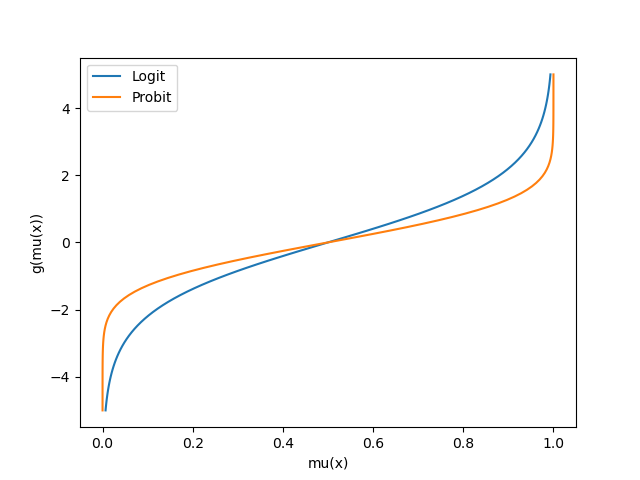
\includegraphics[scale=0.5]{img/probit_logit.png}
            \caption{Logit and Probit Functions}
            \label{fig:logit_probit}
        \end{figure}
    \end{enumerate}
    \end{example}

    Now there are many choices of functions we can take. In fact, if $\mu$ lives in $(0, 1)$, then we can really just take our favorite distribution that has a density that is supported everywhere in $\mathbb{R}$ and take the inverse cdf as our link. So far, we have no reason to prefer one function to another, but in the next section, we will see that there are more natural choices. 

    \subsubsection{Canonical Link Functions}

      Now let's summarize what we have. We assume that the conditional distribution $Y \mid X = x$ follows a distribution in the exponential family, which we can completely characterize by the cumulant generating function $\psi$. For different values of $x$, the conditional distribution will be paramaterized by different $\eta (x)$, and the resulting distribution $P_\eta$ will have some mean $\mu(x)$, which is usually not the natural parameter $\eta$. Now, let's forget about our knowledge that $\psi^\prime(\eta) = \mu$, but we know that there is some relationship between $\eta \leftrightarrow \mu$.

      Given an $x$, I need to use the linear predictor $x^T \beta$ to predict $\mu(x)$, which can be done through the link function $g$. 
      \[g\big( \mu(x) \big) = x^T \beta\]
      Now what would be a natural way of choosing this $g$? Note that our natural parameter $\eta$ for this canonical family takes value on the entire real line. I must construct a function $g$ that maps $\mu$ onto the entire real line, and so why not make it map to $\eta$. Therefore, we have 
      \[\eta(x) = g\big( \mu(x) \big) = x^T \beta\]

      \begin{definition}[Canonical Link]
      The function $g$ that links the mean $\mu$ to the canonical parameter $\theta$ is called the \textbf{canonical link}. 
      \[g(\mu) = \theta\]
      Now using our knowledge that $\psi^\prime(\eta) = \mu$, we can see that 
      \[g = (\psi^\prime)^{-1}\]
      This is indeed a valid link function. 
      \begin{enumerate}
          \item $\psi^{\prime\prime} > 0$ since it models the variance, and so $\psi^\prime$ is strictly increasing and so $g = (\psi^\prime)^{-1}$ is also strictly increasing. 
          \item The domain of $\psi^\prime$ is the real line since it takes in the natural parameter $\eta$ which exists over $\mathbb{R}$, so $\mathrm{Im}(g) = \mathbb{R}$. 
      \end{enumerate}
      \end{definition}

      So, given our cumulant generating function $\psi$ and our link function $g$, both satisfying 
      \[\psi^\prime (\eta) = \mu \text{ and } g(\mu) = x^T \beta\]
      we can combine them to get 
      \[(g \circ \psi^\prime) (\eta) = g(\mu) = x^T \beta\]
      and so, even though the mean of the response variable is not linear with respect to $x$, the value of $(g \circ \psi^\prime) (\eta)$ is indeed linear. In fact, if we choose the canonical link, then the equation 
      \[\eta = x^T \beta\]
      means that the natural parameter of our conditional distribution in the exponential family is linear with respect to $x$! From this we can find the conditional mean $\mu(x)$. 

      The reason we focus on canonical link functions is because, when the canonical link is used, the components of the model (the parameters of the linear predictor) have an additive effect on the response variable in the transformed (linked) scale, which makes the interpretation of the results easier. It's also worth noting that while using the canonical link function has some desirable properties, it is not always the best or only choice, and other link functions may be used if they provide a better fit for the data or make more sense in the context of the problem at hand.

      Let us evaluate some canonical link functions. 

      \begin{example}
      The Bernoulli has the canonical exponential form of 
      \[p_\eta (x) = \exp \big[ x \eta - \log (1 + e^\eta) \big]\]
      where $\eta = \log \big( \frac{\theta}{1 - \theta} \big)$. Since we have prior knowledge that $\theta = \mu$ (i.e. the expectation of a Bernoulli is the hyperparameter $\theta$ itself), we have a function that maps $\mu \mapsto \eta$. 
      \[\eta = g(\mu) = \log \bigg( \frac{\mu}{1 - \mu} \bigg)\]
      which gives us our result. We can also take the inverse of $\psi^\prime = \frac{e^\eta}{1 + e^\eta}$ to get our result 
      \[g (\mu) = (\psi^\prime)^{-1} (\mu) = \log \bigg( \frac{\mu}{1 - \mu} \bigg) \]
      \end{example}

  \subsection{Likelihood Optimization}

    Now let us have a bunch of data points $\{(x_n, y_n)\}_{n=1}^N$. By our model assumption, we know that the conditional distribution $Y \mid X = x_n$ is now of an exponential family with parameter $\eta_n = \eta (x_n)$ and density 
    \[p_{\eta_n} (y_n) = \exp \big[ y_n \eta_n - \psi(\eta_n) \big] h(y_n)\]
    Now we want to do likelihood optimization on $\beta$ (not $\eta$ or $\mu$), and to do this, we must rewrite the density function in a way so that it depends on $\beta$. Given a link function $g$, note the following relationship between $\beta$ and $\eta$: 
    \begin{align*}
        \eta_n = \eta (x_n) & = (\psi^\prime)^{-1} (\mu (x_n)) \\
        & = (\psi^{\prime})^{-1} \big( g^{-1} (x_n^T \beta )\big) \\
        & = h(x_n^T \beta) 
    \end{align*}
    where for shorthand notation, we define $h \coloneqq (g \circ \psi^\prime)^{-1}$. Subtituting this into the above likelihood, taking the product of all $N$ samples, and logarithming the equation gives us the following log likelihood to optimize over $\beta$. 
    \[\ell(\beta) = \log \prod_{n=1}^N p_{\eta_n} (y_n) = \sum_{n=1}^N y_n h(x_n^T \beta)  - \psi(h(x_n^T \beta) )\]
    where we dropped the $h(y_n)$ term at the end since it is a constant and does not matter. If $g$ was the canonical link, then $h$ is the identity, and we should have a linear relationship between $\eta (x_n) = x_n^T \beta$. This means that the $\eta_n$ reduces only to $x_n^T \beta$, which is much more simple to optimize. 
    \[\ell(\beta) = \log \prod_{n=1}^N p_{\eta_n} (y_n) = \sum_{n=1}^N y_n x_n^T \beta - \psi(x_n^T \beta)\]
    Note that the first term is linear w.r.t $\beta$, and $\psi$ is convex, so the entire sum must be concave w.r.t. $\beta$. With this, we can bring in some tools of convex optimization to solve. 

